\maketitle
\tableofcontents
\newpage

\section{Zielsetzung}
Ziel dieses Versuches ist es, das Relaxationsverhalten eines RC-Gliedes zu
untersuchen. Dabei wird die Zeitkonstante des Kreises bestimmt, die Amplitude
der Kondensatorspannung und die Phasenverschiebung zwischen Generator- und Kondensatorspannung
in Abhängigkeit von der Frequenz aufgenommen und ermittelt, unter welchen Vorraussetzungen
ein RC-Kreis als Integrator genutzt werden kann.
\section{Theorie}
\subsection{Relaxationserscheinungen ohne Periodizität}
\label{sec:2.1}
Wenn ein System aus seinem Ausgangszustand entfernt wird und ihn nicht mittels Ozillation
wieder erreicht, dann spricht man von Relaxation. Dabei ist die Änderungsgeschwindigkeit
der Größe $A$ proportional zu
\begin{equation}
    \frac{\symup dA}{\symup dt} = c \left[A(t) - A(\infty) \right]
    \label{eqn:1}
\end{equation}
mit $t = bel.$ und $A(\infty)$ der Endzustand des Systems. Wenn \eqref{eqn:1} über
die Zeitpunkte 0 bis $t$ integriert wird, folgt
\begin{equation}
    A(t) = A(\infty) + \left[A(0) - A(\infty) \right] e^{\, ct} \, .
    \label{eqn:2}
\end{equation}
Damit \eqref{eqn:2} beschränkt bleibt, muss $c < 0$ gelten. Als Beispiel für
solche Relaxationsvorgänge lässt sich das Auf- und Entladen eines Kondensators
über einen Widerstand nennen. Eine passende Schaltung ist in Abbildung \ref{fig:1}
dargestellt.
\begin{figure}
  \centering
  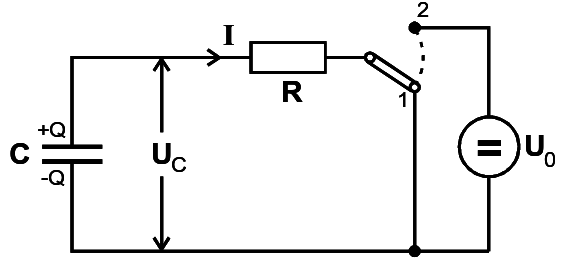
\includegraphics[scale=0.5]{kondensator.png}
  \caption{Schaltskizze zum Auf- (Stellung 2) und Entladen (Stellung 1) eines
  Kondensators \cite{anleitung}.}
  \label{fig:1}
\end{figure}
\begin{itemize}
  \item \textbf{Entladevorgang}:

  Es wird angenomen, dass zum Zeitpunkt $t = 0$ die Ladung $Q$ auf dem Kondensator
  mit der Kapazität $C$ liegt. Damit folgt für die Spannung
  \begin{equation*}
    U_\symup{C} = \frac{Q}{C} \, .
  \end{equation*}
  Unter Zuhilfenahme des ohmschen Gesetztes und der Beziehung zwischen zeitlicher Änderung
  deR Ladung in Relation zum Strom ergibt sich eine Differentialgleichung nach Gestalt
  von \eqref{eqn:1}. Wenn man annimmt, dass nach unendlicher langer Zeit der Kondensator vollständig
  entladen ist, und ersetzt in \eqref{eqn:2} $U(\infty)$ mit 0, dann folgt
  \begin{equation}
    Q(t) = Q(0) e^{-\frac{t}{RC}} \, .
    \label{eqn:3}
  \end{equation}

  \item \textbf{Aufladevorgang}:

  Nach dem gleichen Prinzip erfolgt die Aufladung eines Kondensators; diesmal mit
  den Randbedingungen
  \begin{align*}
      Q(0) &= 0 \\
      Q(\infty) &= C U_0 \, .
  \end{align*}
  Damit folgt eine Gleichung ähnlich zu \eqref{eqn:3} nach Gestalt von \eqref{eqn:2}
  \begin{equation}
    Q(t) = C U_0 \left(1 - e^{-\frac{t}{RC}} \right) \, ,
    \label{eqn:4}
  \end{equation}
  wobei der Ausdruck $RC$ als Zeitkonstante bezeichnet wird. Diese Zeitkonstante
  liefert eiine Aussage über die Geschwindigkeit mit der der Endzustand erreicht wird.
\end{itemize}

\subsection{Relaxationserscheinungen mit Periodizität und RC-Glied als Integrator}
Relaxationsvorgänge treten auch auf, wenn das System periodisch ausgelenkt wird. Um
dies zu untersuchen, wird der Schaltplan aus Abbildung \ref{fig:1} nun um einen
Wechselstromgenerator erweitert, der eine sinusförmige Spannung mit
\begin{equation}
    U(t) = U_0 \, \symup{cos} \left(\omega t \right)
    \label{eqn:5}
\end{equation}
liefert. Ein solcher Schaltplan ist in Abbildung \ref{fig:2} zu sehen.
\begin{figure}
  \centering
  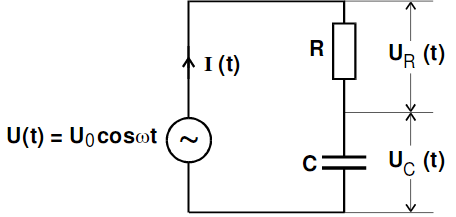
\includegraphics[scale=0.6]{kondensator2.png}
  \caption{Schaltskizze zur Untersuchung von Relaxationserscheinungen bei
  periodischen Auslenkungen. \cite{anleitung}}
  \label{fig:2}
\end{figure}
Solange in \eqref{eqn:5} $\omega << 1/(RC)$ gilt, kann man annehmen, dass die Spannung
am Kondensator zu jeder Zeit praktisch gleich $U(t)$ ist. Wenn nun $\omega$ größer
wird, dann wird sich eine Phase $\phi$ zwischen Kondensator- und Generatorspannung
bilden und die Amplitude $A$ der Kondensatorspannung wird sinken. Zur weiteren
Untersuchung des Phänomens lässt sich mit dem Ansatz
\begin{equation}
    U_\symup{C}(t) = A(\omega) \, \symup{cos} \left[\omega t + \phi (\omega)  \right]
    \label{eqn:6}
\end{equation}
ein Ausdruck für die Frequenzanhängigkeit der Phase
\begin{equation}
  \phi (\omega) = \symup{arctan} \left(- \omega RC \right)
  \label{eqn:7}
\end{equation}
finden. An \eqref{eqn:7} lässt sich bestätigen, dass die Phasenverschiebung für
kleine $\omega$ gegen 0 und für große gegen $\frac{\pi}{2}$ geht. Für die Amplitude
$A$ in Abhängigkeit von der Frequenz ergibt sich
\begin{equation}
    A(\omega) = \frac{U_0}{\sqrt{1 + \omega^2 R^2 C^2}} \, .
    \label{eqn:8}
\end{equation}
Die Amplitude $A(\omega)$ geht für $\omega \to 0$ gegen $U_0$ und für
$\omega \to \infty$ gegen 0; so wie bereits diskutiert. Aus diesem Grund wird
ein RC-Kreis oft als Tiefpass verwendet.

Unter der Vorraussetzung, dass $\omega$ gegenüber $\frac{1}{RC}$ viel größer ist,
kann ein RC-Glied auch die angelegte Spannung $U(t)$ integrieren. In diesem Fall
gilt näherungsweise
\begin{equation}
    U_\symup{C} (t) = \frac{1}{RC} \int_0^t U(t') \symup d t' \, .
    \label{eqn:9}
\end{equation}

\section{Durchführung}
\subsection{Versuchsaufbau}
\begin{figure}
  \centering
  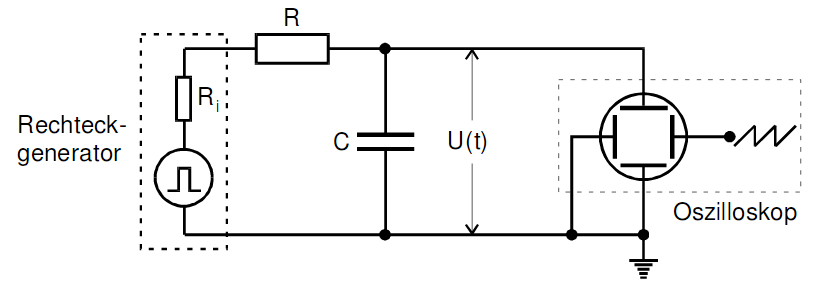
\includegraphics[scale=0.4]{aufbau.png}
  \caption{Schaltplan zur Versuchsdurchführung. \cite{anleitung}}
  \label{fig:3}
\end{figure}
In Abbildung \ref{fig:3} ist der Schaltplan dargestellt, der für alle Teile der Versuchsdurchführung
nutzbar ist. Dabei ist zu beachten, dass der Rechteckgenerator in unserem Fall durch
einen Funktionsgenerator mit verstellbarer Frequenz ersetzt wurde,
der auch die anderen, für den letzten Teil der Durchführung nötigen Spannungen, liefert. Dieser ist mit einem
nachfolgend geschalteten RC-Glied verbunden, während jener parallel zu einem Zweikanal-Oszilloskop
geschaltet ist. Der zweite Kanal wird für alle Versuchsteile
direkt mit der Generatorspannung verbunden.

\subsection{Versuchsdurchführung}
Im ersten Teil des Versuchs wird die Zeitkonstante aus Kapitel \ref{sec:2.1} aus
der Entladekurve in Abbildung \ref{fig:4} gewonnen, indem acht Datenpaare, die aus
der Zeit und der Kondensatorspannung in Abhängigkeit von der Zeit bestehen, aus
jener Entladekurve abgelesen werden.
\begin{figure}
  \centering
  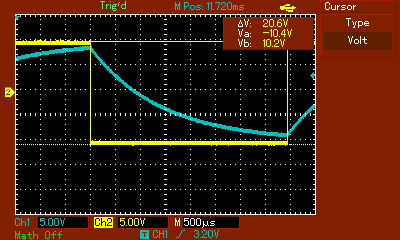
\includegraphics[scale=0.5]{zeitkonstante.png}
  \caption{Entladekurve des Kondensators, aus dem die Zeitkonstante $RC$ gewonnen wird.
  In blau ist die Spannung $U_\symup{C}(t)$ und in gelb die Generatorspannung $U(t)$ aufgetragen.}
  \label{fig:4}
\end{figure}

Im zweiten und dritten Teil werden Amplitude der Kondensatorspannung und Phasenverschiebung
zwischen Kondensator- und Generatorspannung in Abhängigkeit von der Frequenz untersucht.
Dazu wird der Funktionsgenerator auf eine Sinusspannung mit insgesamt elf
Frequenzen im Bereich von 25 bis $\SI{1750}{\hertz}$ am Funktionsgenerator eingestellt.
Dazu wird über die Measure- und Cursor-Funktion des Oszilloskops die Kondensatorspannung
und die Zeitdifferenz zwischen den Nulldurchgängen der beiden Spannungen aufgenommen.

Im letzten Teil werden eine Sinus-, eine Dreiecks, und eine Rechteckspannung
mit jeweils einer Frequenz von $\SI{12.5}{\kilo\hertz}$ über das RC-Glied integriert
und die Spannungenspaare am Oszilloskop als Bilder abgespeichert.

\section{Auswertung}
\subsection{Bestimmen der Zeitkonstante aus dem Relaxationsverhalten der Kondensatorspannung}
\begin{figure}
  \begin{subfigure}{0.74\textwidth}
  \centering
    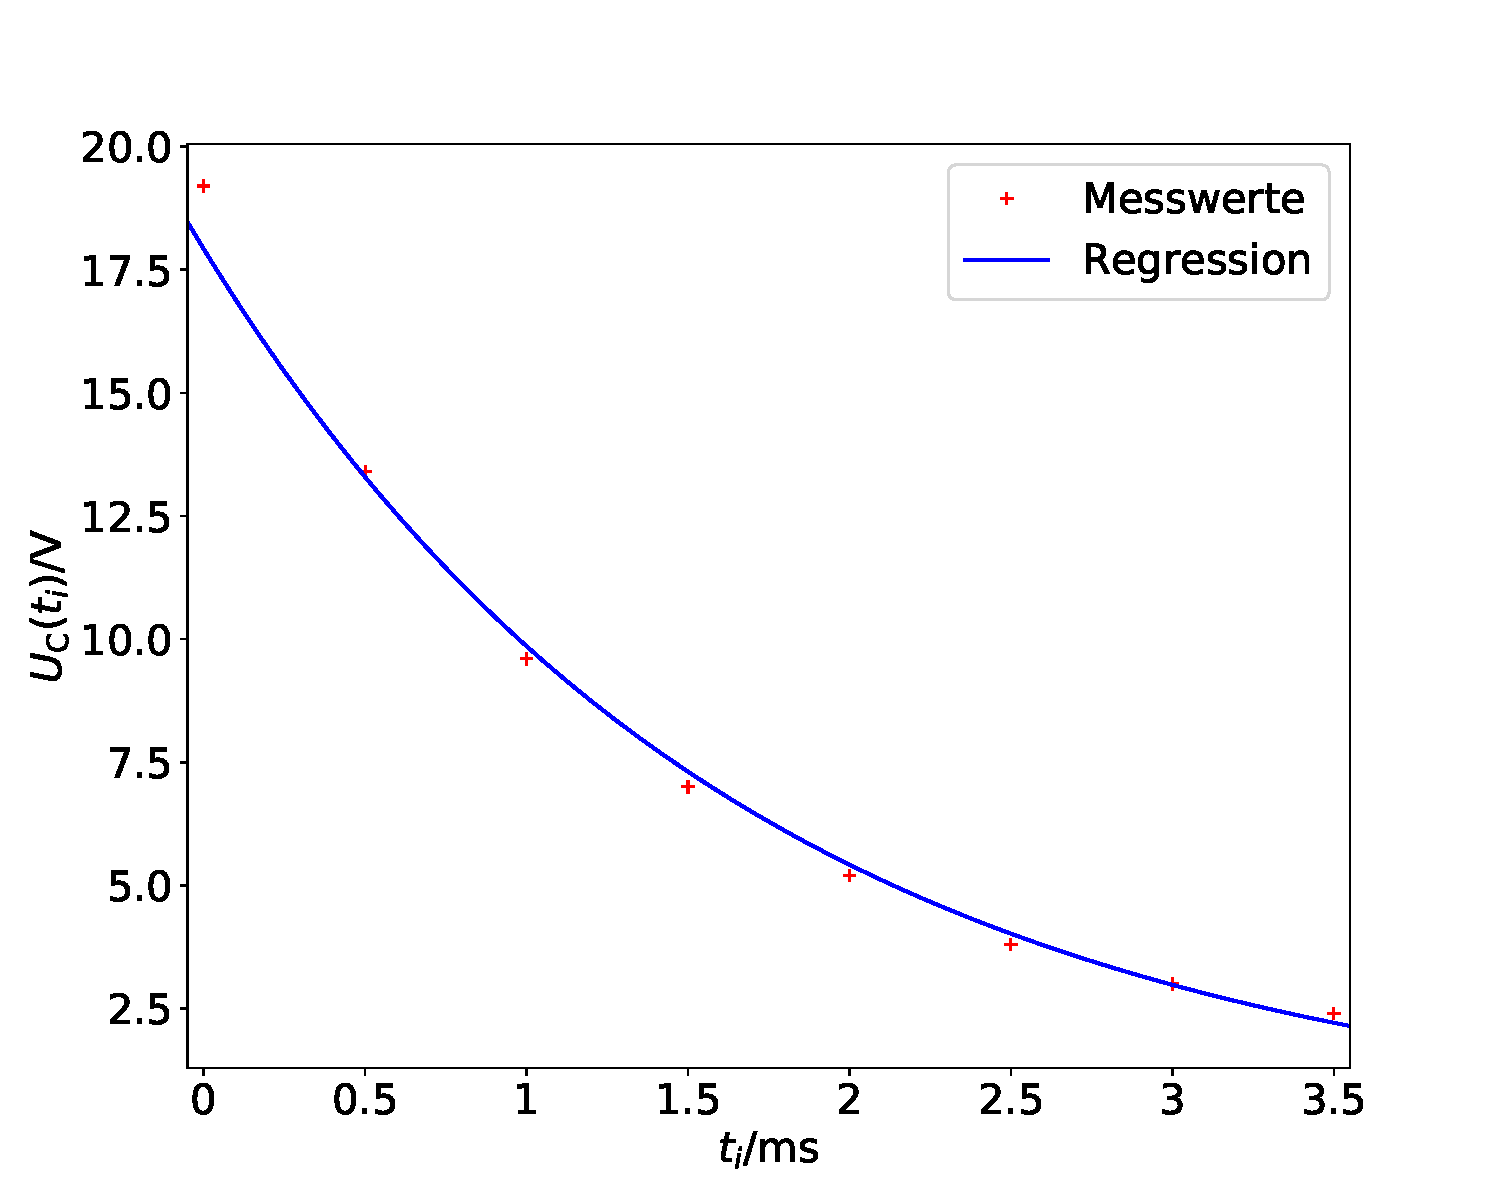
\includegraphics[width=\textwidth]{Entladung.pdf}
    \qquad
  \end{subfigure}
  \begin{subtable}{0.25\textwidth}
  \centering
  \begin{tabular}{c c}
    \toprule
    $t_i$/\si{\milli\second} & $U_\symup{C}(t_i)$/\si{\volt} \\
    \midrule
    0 & 19.2 \\
    0.5 & 13.4 \\
    1 & 9.6 \\
    1.5 & 7 \\
    2 & 5.2 \\
    2.5 & 3.8 \\
    3 & 3 \\
    3.5 & 2.4 \\
    \bottomrule
  \end{tabular}
    \qquad
  \end{subtable}
  \caption{In der Tabelle finden sich die aus der Entladekurve des Kondenators gemessenen zeitabhängige Kondensatorspannungen.
  Diese wurden in der Grafik mit der berechneten Regression dargestellt.}
\label{tab:1}
\end{figure}
Die gemessenen Werte sind mit Graph in Abbildung \ref{tab:1} dargestellt. Zur Bestimmung der Zeitkonstante wird
eine lineare Ausgleichsrechnung durchgeführt. Aus \eqref{eqn:3} folgt mit $\tau = RC$:
\begin{equation}
  \ln({U_\symup{C}}) = \ln({U(0)}) - t \cdot \frac{1}{\tau}.
\end{equation}
Fitten der Wertepare $\{(\ln({U_\symup{C}(t_i)}), t_i)\}$ durch eine Funktion
\begin{equation}
  f(x) = m \cdot x + b
\end{equation}
in "python" mit "curve-fit" aus dem Paket "scipy-optimize" liefert diese Werte für $U(0)$ und die
Zeitkonstante $\tau$:
\begin{align*}
  b &= \ln({U(0)}) = \num{2.89(4)} \\
  m &= -\frac{1}{\tau} = \SI[per-mode=reciprocal]{-598(17)}{\per\second}
\end{align*}
woraus für $U(0)$ und $\tau$ folgt:
\begin{align*}
  U(0) &= \SI{17.9(7)}{\volt} \\
  \tau &= \SI{1.67(5)}{\milli\second}.
\end{align*}
Diese Regression ist ebenfalls in Abbildung \ref{tab:1} dargestellt.
\subsection{Bestimmen der Zeitkonstante aus der Frequenzabhängigkeit der Amplitude der Kondensatorspannung}
\begin{figure}
  \begin{subfigure}{0.74\textwidth}
  \centering
    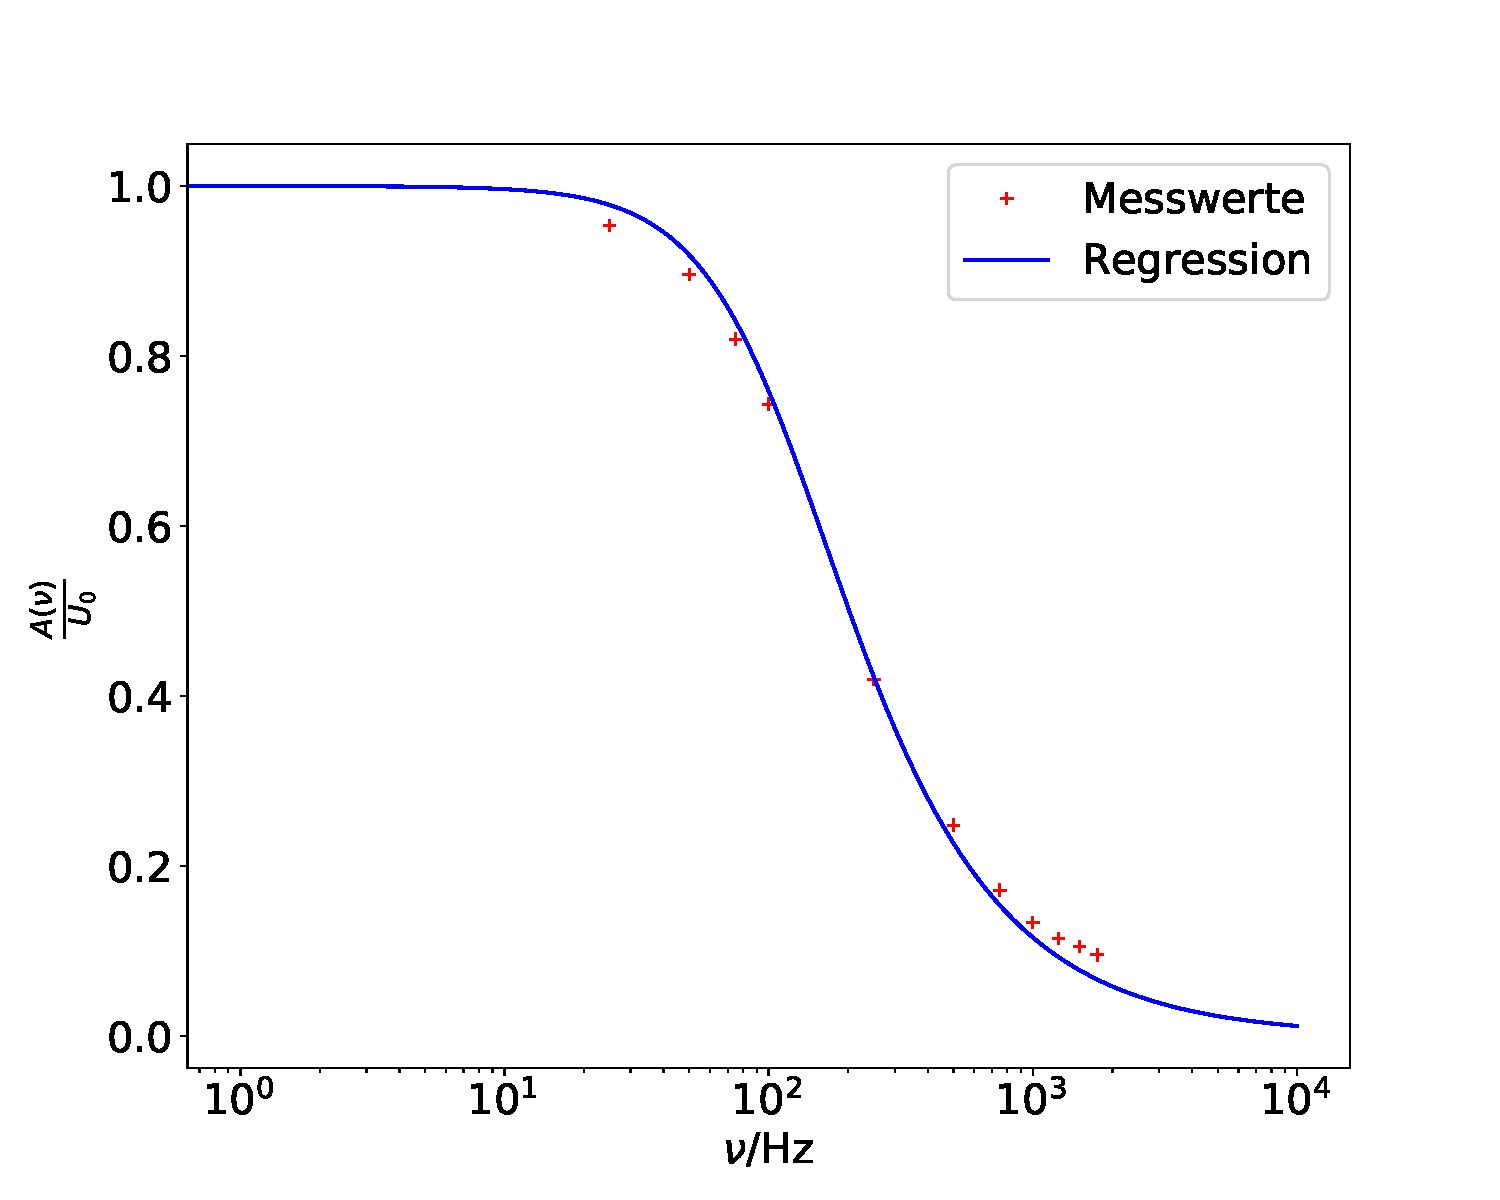
\includegraphics[width=\textwidth]{Amplitude.pdf}
    \qquad
  \end{subfigure}
  \begin{subtable}{0.25\textwidth}
  \centering
  \begin{tabular}{c c}
    \toprule
    $\nu$/\si{\hertz} & $U_\symup{C}$/\si{\volt}\\
    \midrule
    25 & 19.80 \\
    50 & 18.61 \\
    75 & 17.03 \\
    100 & 15.44 \\
    250 & 8.71 \\
    500 & 5.15 \\
    750 & 3.56 \\
    1000 & 2.77 \\
    1250 & 2.38 \\
    1500 & 2.18 \\
    1750 & 1.98 \\
    \bottomrule
    \end{tabular}
    \qquad
  \end{subtable}
  \caption{In der Tabelle sind die gemessenen Amplituden der Kondensatorspannung bei
  verschiedenen Frequenzen aufgeführt. Diese wurden in der Grafik in halblogarithmischer
  Darstellung gegeneinander abgetragen. Die Amplituden wurden dazu mit der konstanten,
  gemessenen Spannung $U_0 = \SI{20.77}{\volt}$ normiert. Zusätzlich wurde eine Regressionsgerade eingezeichnet.}
\label{abb:1}
\end{figure}
Messwerte und Grafik sind in Abbildung \ref{abb:1} dargestellt. Die Regression ergibt sich
durch Ausgleichsrechnung nach \eqref{eqn:8}. Für die Zeitkonstante folgt dabei ein Wert von:
\begin{align*}
  \tau &= \SI{1.37(5)}{\milli\second}.
\end{align*}
Die Regression verhält sich wie zu erwarten. Für geringe Frequenzen zeigt sich das normale
Verhalten eines Kondensators. Für $\nu \mapsto \infty$ "schaltet" der Kondensator jedoch durch
und verhält sich wie ein normales Leitungsstück, sodass keine Spannung mehr am Kondensator messbar ist.
\subsection{Bestimmen der Zeitkonstante aus der Frequenzabhängigkeit der Phase zwischen Kondensator-
und Erregerspannung}
\begin{figure}
  \begin{subfigure}{0.74\textwidth}
  \centering
    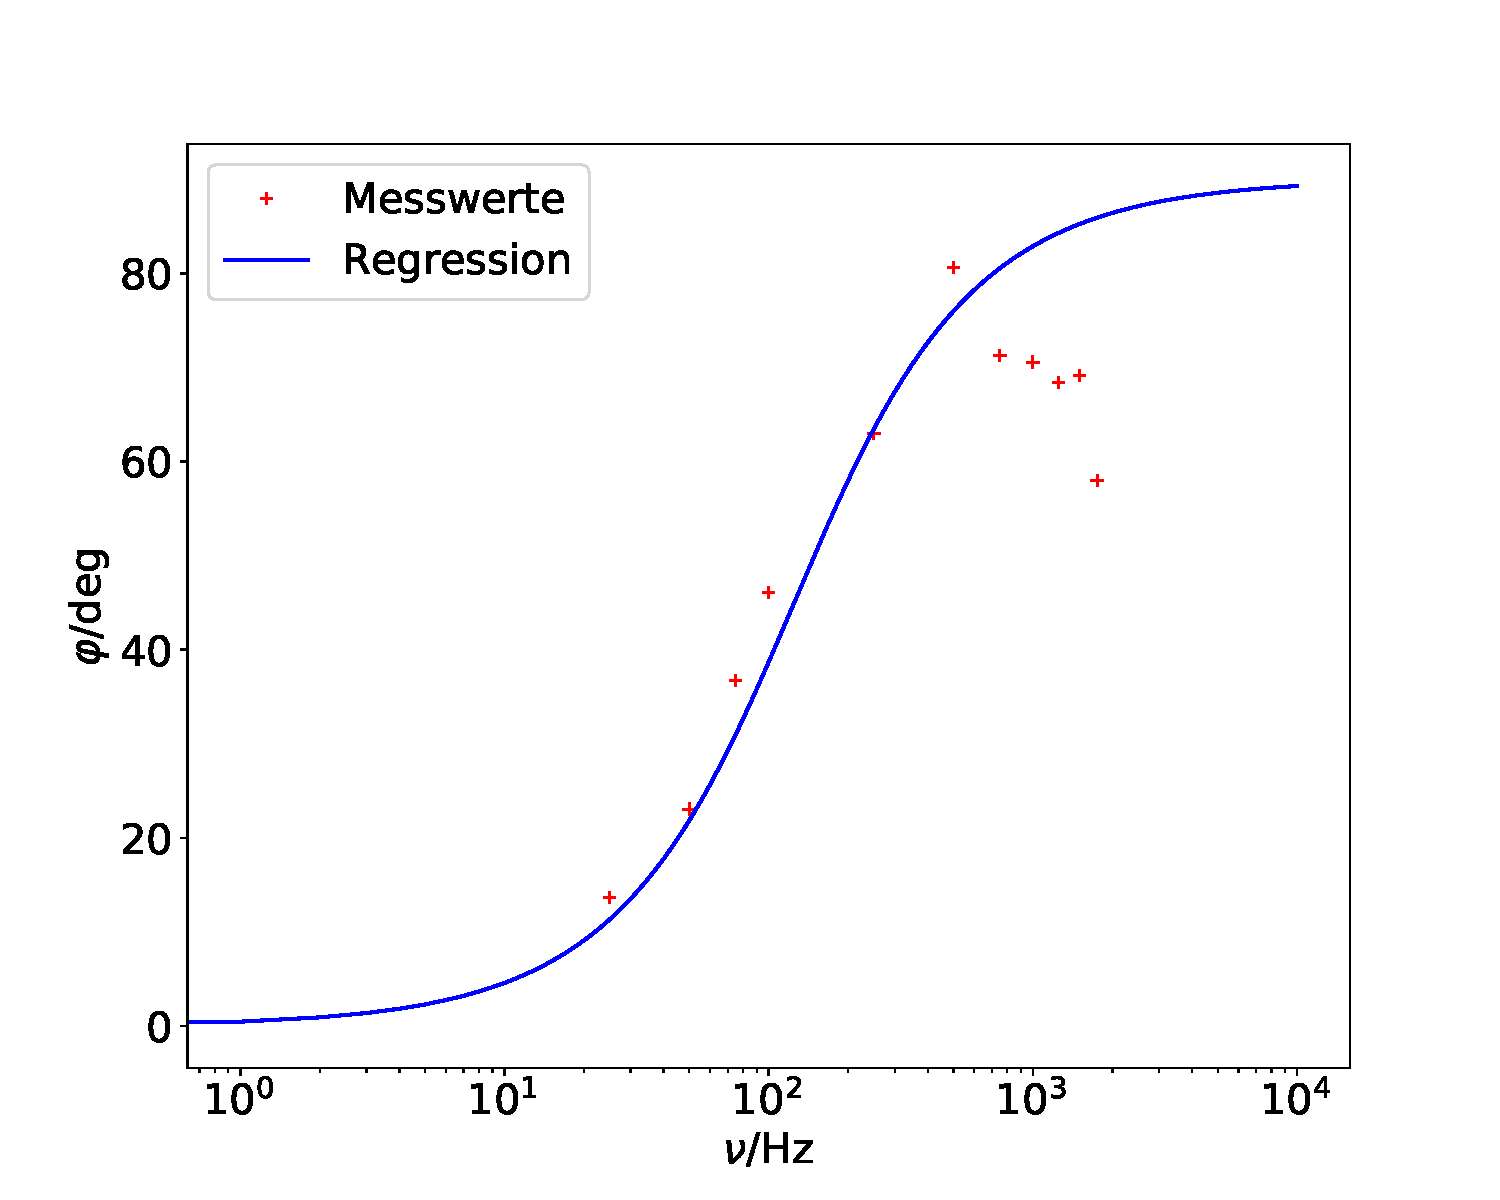
\includegraphics[width=\textwidth]{Phase.pdf}
    \qquad
  \end{subfigure}
  \begin{subtable}{0.25\textwidth}
  \centering
  \begin{tabular}{c c c}
    \toprule
    $\nu$/\si{\hertz} & $\symup{\Delta}t$/\si{\milli\second} & $\varphi$/deg\\
    \midrule
    25 & 1.520 & 13.7 \\
    50 & 1.280 & 23.0 \\
    75 & 1.360 & 36.7 \\
    100 & 1.280 & 46.1 \\
    250 & 0.700 & 63.0 \\
    500 & 0.448 & 80.6 \\
    750 & 0.264 & 71.3 \\
    1000 & 0.196 & 70.6 \\
    1250 & 0.152 & 68.4 \\
    1500 & 0.128 & 69.1 \\
    1750 & 0.092 & 58.0 \\
    \bottomrule
    \end{tabular}
    \qquad
  \end{subtable}
  \caption{In der Tabelle sind die gemessenen Zeitverschiebungen zwischen Kondensator- und
  Erregerspannung bei verschiedenen Frequenzen sowie die daraus berechnete Phase
  eingetragen. In der Grafik wurde die Phase gegen
  die Frequenz in halblogarithmischer Darstellung abgetragen.
  Zusätzlich wurde eine Regressionsgerade eingezeichnet.}
\label{abb:2}
\end{figure}
Messwerte und Grafik sind in Abbildung \ref{abb:2} dargestellt. Die Phasen ergeben sich nach
\begin{equation}
  \varphi = \frac{\symup{\Delta}t}{T} \cdot 360
\end{equation} mit der Periodendauer $T=\nu^{-1}$. Die Regression ergibt
nach \eqref{eqn:7} eine Zeitkonstante von:
\begin{align*}
  \tau &= \SI{1.28(31)}{\milli\second}.
\end{align*}
Zur besseren Darstellung findet sich in Abbildung \ref{abb:3} eine Polardarstellung der
Phasen mit einer Theoriekurve.
\begin{figure}
  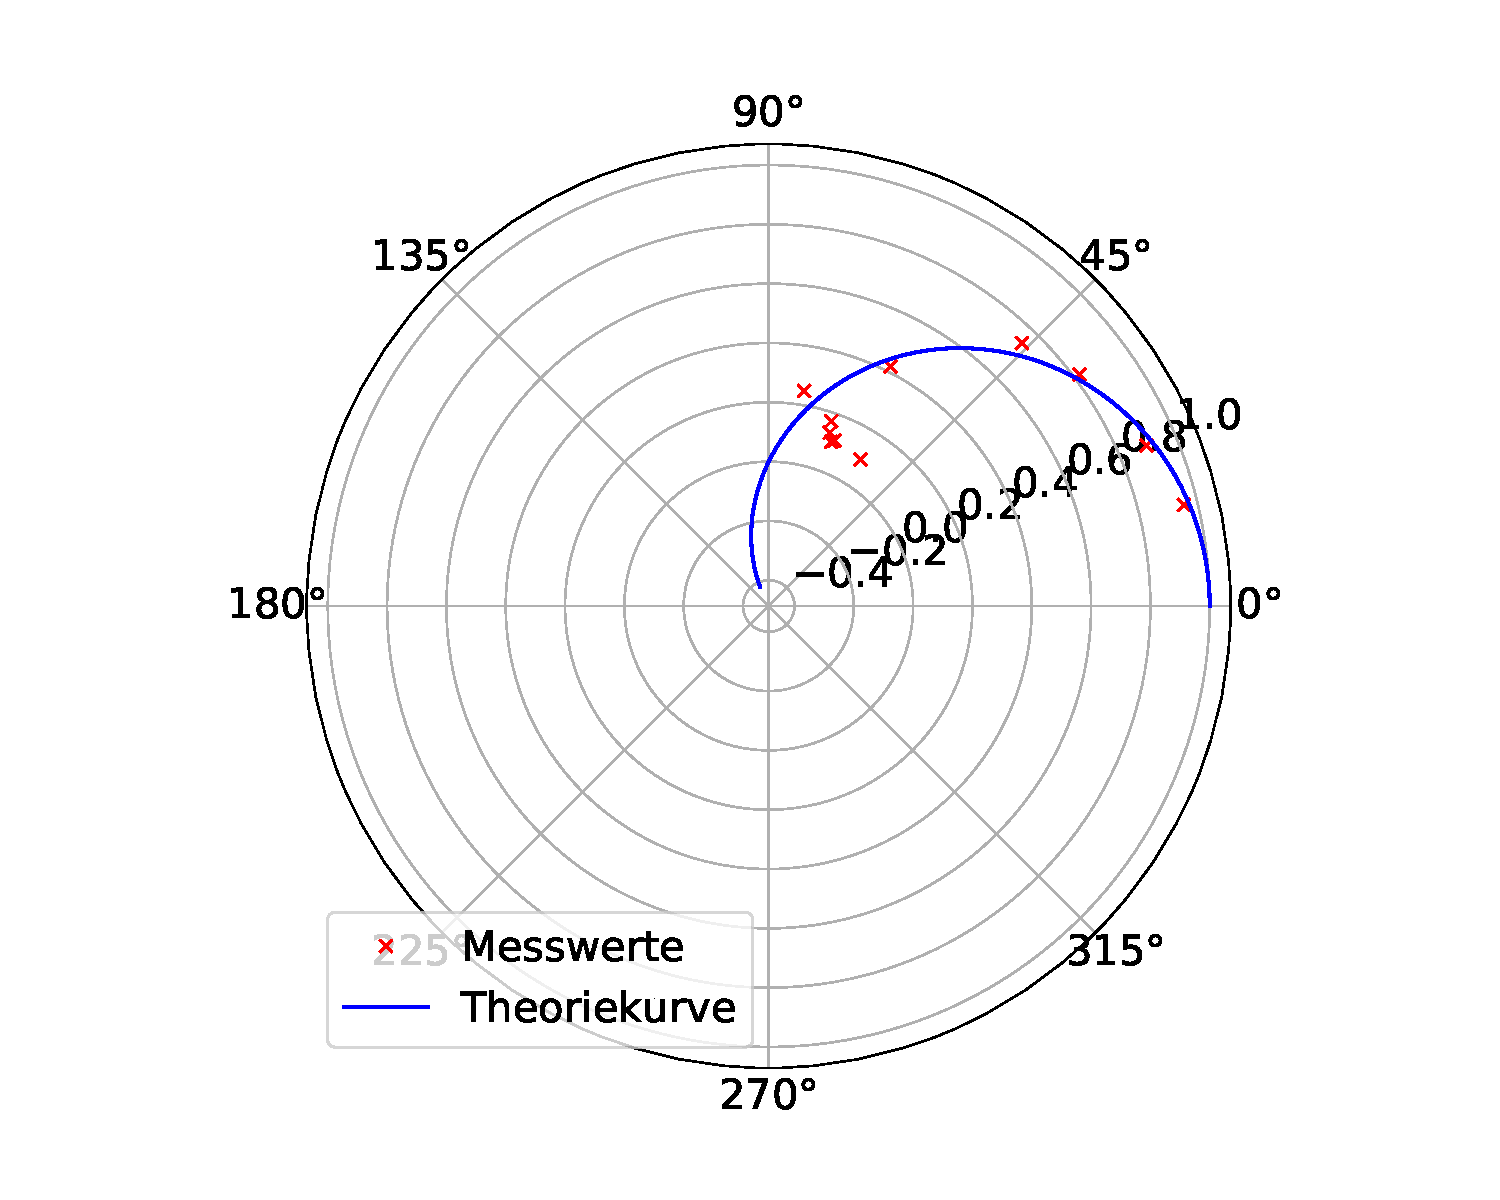
\includegraphics[width=\textwidth]{Polar.pdf}
  \caption{Polardarstellung der Phasen mit Theoriekurve.}
  \label{abb:3}
\end{figure}
\subsection{Der RC-Kreis als Intergrationsglied}
Zum Integrieren wurde eine Frequenz von \SI{12.5}{\kilo\hertz} am Funktionsgenerator
eingestellt. Es ergeben sich die in Abbildung \ref{abb:4} dargestellten Bilder auf
dem Oszilloskop. Theoretisch liefert die Integration einer Rechteckfunktion (Abbildung \ref{sub:1}) eine
Dreieckfunktion, die Integration einer Dreieckfunktion (Abbildung \ref{sub:2}) eine parabelförmige Funktion
und die Integration eines Sinus (Abbildung \ref{sub:3}) einen Cosinus. Dies entspricht den erhaltenen Ergebnissen.
\begin{figure}
  \begin{subfigure}{0.49\textwidth}
  \centering
    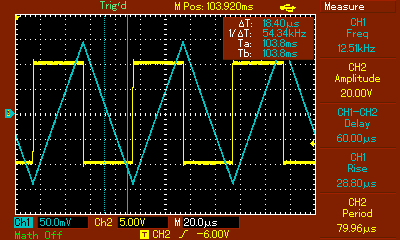
\includegraphics[width=\textwidth]{rechteck.png}
    \qquad
    \caption{Integration einer Rechteckspannung.}
    \label{sub:1}
  \end{subfigure}
  \begin{subfigure}{0.49\textwidth}
  \centering
    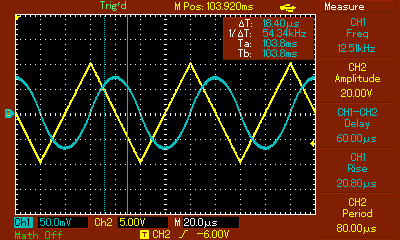
\includegraphics[width=\textwidth]{dreieck.png}
    \qquad
    \caption{Integration einer Dreieckspannung.}
    \label{sub:2}
  \end{subfigure}\\
  \begin{subfigure}{0.49\textwidth}
  \centering
    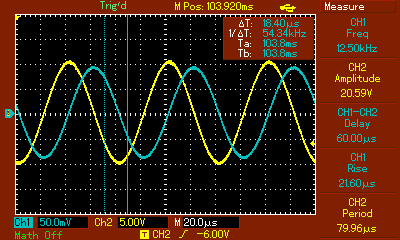
\includegraphics[width=\textwidth]{sinus.png}
    \qquad
    \caption{Integration einer Sinusspannung.}
    \label{sub:3}
  \end{subfigure}
  \caption{Oszilloskopbilder nach Integration der verschiedenen Spannungsformen.
  Die Erregerspannungen sind in gelb dargestellt, die erhaltenen Signalspannungen in blau.}
\label{abb:4}
\end{figure}
\section{Diskussion}
\begin{table}
  \centering
  \begin{tabular}{c c c c}
    \toprule
    & Direkt & Amplitude & Phase \\
    \midrule
    $\tau$/\si{\milli\second} & \num{1.67(5)} & \num{1.37(5)} &\num{1.28(31)} \\
    \bottomrule
  \end{tabular}
  \caption{Gegenüberstellung der bestimmten Zeitkonstanten aus den unterschiedlichen Messmethoden.
  Direkt steht dabei für die Bestimmung aus dem Relaxationsverhalten des RC-Kreises, Amplitude
  und Phase für die Bestimmungen aus dem jeweiligen Frequenzverhalten.}
  \label{tab:2}
\end{table}
In Tabelle \ref{tab:2} sind die Ergebnisse der einzellnen Methoden zusammengefasst.
Auffällig ist das große Fehlerintervall der Phasenmessung. Dies erscheint bei Betrachtung
der Messwerte logisch. Die bestimmten Phasen verhalten sich ab einem gewissen Punkt
nicht mehr wie ein arccos (siehe Abbildung \ref{abb:3}). Der Grund ist hier nicht
abschließend zu klären. Messfehler durch die Art der Auswertung durch das manuelle
Setzen von Zeigern sind möglich, müssten aber alle Messwerte ähnlich stark betreffen
und sollten nicht gehäuft bei Messungen hoher Frequenzen auftreten. Generell ist bei
allen Messungen mit systematischen Fehlern zu rechnen, da der Innenwiderstand des
Funktionsgenerators nicht berücksichtigt wird. Desweiteren kann kein Messwert mit einem
aus Bauteilwerten bestimmten Theoriewert verifiziert werden, da keine Bauteilwerte
angegeben werden. Um sinnvolle Aussagen über den Wert der Ergebnisse treffen zu können, wäre
dementsprechend ein Durchmessen der Bauteile nötig, um Vergleiche zu einem
Theoriewert ziehen zu können.
\newpage
\nocite{*}
\printbibliography
